% ------------------------------------------------------------------------------
% TYPO3 Version 10.0 - What's New (English Version)
%
% @author	Michael Schams <schams.net>
% @license	Creative Commons BY-NC-SA 3.0
% @link		http://typo3.org/download/release-notes/whats-new/
% @language	English
% ------------------------------------------------------------------------------

\section{Changes for Developers}
\begin{frame}[fragile]
	\frametitle{Changes for Developers}

	\begin{center}\huge{Chapter 4:}\end{center}
	\begin{center}\huge{\color{typo3darkgrey}\textbf{Changes for Developers}}\end{center}

\end{frame}

% ------------------------------------------------------------------------------
% TYPO3 Version 10.0 - Breaking Changes

\begin{frame}[fragile]
	\frametitle{Changes for Integrators}
	\framesubtitle{Breaking Changes}

	\small
		Developers be advised: In TYPO3 v9, some PHP classes, interfaces, class aliases,
		properties, methods, constants, global options and variables, etc. were marked
		deprecated.

		\vspace{0.2cm}

		In accordance to TYPO3's \textbf{deprecation policy}, these components have
		been removed in TYPO3 v10.0.

		\vspace{0.2cm}

		This also includes some hooks, PHP annotations (such as \texttt{@inject} and
		\texttt{@validate}), as well as some changed visibilities (e.g. from
		"\texttt{public}" to "\texttt{protected}").

		\vspace{0.2cm}

		Enable the deprecation log, carefully test your code and review the log to
		locate possible issues. Use the built-in
		\href{https://docs.typo3.org/m/typo3/reference-coreapi/master/en-us/ApiOverview/ExtensionScanner/Index.html}{Extension Scanner}
		to get a full report of extension incompatibilities.

	\normalsize

\end{frame}

% ------------------------------------------------------------------------------
% Feature | 88643 | New Mail API based on symfony/mailer and symfony/mime
% Breaking | 88643 | Removed Swiftmailerswiftmailer Dependency

\begin{frame}[fragile]
	\frametitle{Changes for Developers}
	\framesubtitle{New Mail API}

	\begin{itemize}
		\item SwiftMailer has been superseded by more modern libraries:

			\begin{itemize}
				\item \texttt{symfony/mime} for creating mail messages
				\item \texttt{symfony/mailer} for sending emails
			\end{itemize}

		\item PHP function \texttt{mail()} is no longer supported.

			\begin{itemize}\smaller
				\item[\ding{228}] It is recommended to switch to \texttt{sendmail} or \texttt{smtp} instead.
			\end{itemize}\normalsize

		\item Custom SwiftMailer plugins or transports require a migration.

		\item See the \href{https://symfony.com/doc/current/mailer.html}{Symfony Documentation}
			for further details how to leverage the new Mail API capabilities.
	\end{itemize}

\end{frame}

% ------------------------------------------------------------------------------
% Feature | 84112 | Symfony dependency injection for core and Extbase

\begin{frame}[fragile]
	\frametitle{Changes for Developers}
	\framesubtitle{Symfony Dependency Management/Injection (1)}

	\begin{itemize}
		\item The package \texttt{symfony/dependency-injection} has been integrated
			and is used to manage system-wide dependency management and dependency
			injection for classes.

		\item This approach aims to replace the Extbase dependency injection
			container and object manager.

		\item Therefore, classes should be adjusted and avoid (whenever possible):

			\begin{itemize}\small
				\item \texttt{\textbackslash
					TYPO3\textbackslash
					CMS\textbackslash
					Extbase\textbackslash
					Object\textbackslash
					ObjectManager}
				\item \texttt{\textbackslash
					TYPO3\textbackslash
					CMS\textbackslash
					Core\textbackslash
					Utility\textbackslash
					GeneralUtility::makeInstance()}
			\end{itemize}\normalsize

	\end{itemize}

\end{frame}

% ------------------------------------------------------------------------------
% Feature | 84112 | Symfony dependency injection for core and Extbase

\begin{frame}[fragile]
	\frametitle{Changes for Developers}
	\framesubtitle{Symfony Dependency Management/Injection (2)}

	% decrease font size for code listing
	\lstset{basicstyle=\tiny\ttfamily}

	\begin{itemize}
		\item Configuration options include:

			\begin{itemize}
				\item Autowiring (see example below)
				\item Manual wiring
					(see \href{https://docs.typo3.org/c/typo3/cms-core/master/en-us/Changelog/10.0/Feature-84112-SymfonyDependencyInjectionForCoreAndExtbase.html}{change log})
				\item Advanced functionality
					(see \href{https://docs.typo3.org/c/typo3/cms-core/master/en-us/Changelog/10.0/Feature-84112-SymfonyDependencyInjectionForCoreAndExtbase.html}{change log})
			\end{itemize}

		% \smaller For example "autowiring":\normalsize

\begin{lstlisting}
# Configuration/Services.yaml
services:
  _defaults:
    autowire: true
    autoconfigure: true
    public: false

  Your\Namespace\:
    resource: '../Classes/*'
\end{lstlisting}

		\item See \href{https://symfony.com/doc/current/service_container.html}{Symfony documentation} for further details.

	\end{itemize}

\end{frame}

% ------------------------------------------------------------------------------
% Feature | 88769 | Introduce a generic EventDispatcher based on PSR-14
% Feature | 88770 | Add PSR-14 EventDispatcher logic based on DI

\begin{frame}[fragile]
	\frametitle{Changes for Developers}
	\framesubtitle{Event Dispatching (1)}

	\begin{itemize}
		\item A new "EventDispatcher" system has been added which aims to replace
			the hooks and Signal/Slots concepts.

		\item It is based on the \href{https://www.php-fig.org/psr/psr-14}{PSR-14 standard}
			which allows developers to inject logic into an application easily and consistently.

		\item PSR-14 consists of the following four components:

			\begin{itemize}
				\item An \textbf{EventDispatcher} object that is used to trigger an event.
				\item A \textbf{ListenerProvider} object that contains registered listeners for all events.
				\item One or multiple \textbf{Event} objects which are called from the TYPO3 core or extensions ("Emitter").
				\item One or multiple \textbf{Listeners} (usually in extensions and PHP packages) that are registered.
			\end{itemize}

% Short-Term goal is to deprecate SignalSlot dispatcher in TYPO3 v10,
% and migrate all signals to the EventDispatcher.

	\end{itemize}

\end{frame}

% ------------------------------------------------------------------------------
% Feature | 88769 | Introduce a generic EventDispatcher based on PSR-14
% Feature | 88770 | Add PSR-14 EventDispatcher logic based on DI

\begin{frame}[fragile]
	\frametitle{Changes for Developers}
	\framesubtitle{Event Dispatching (2)}

	% decrease font size for code listing
	\lstset{basicstyle=\tiny\ttfamily}

	Implementation example

	\begin{itemize}\smaller
		\item[\ding{202}] Add \texttt{event.listener} tag to the file \texttt{Configuration/Services.yaml}:

\begin{lstlisting}
services:
  Vendor\Example\EventListener\NullMailer:
    tags:
      - { name: event.listener, identifier: 'myListener', event: TYPO3\CMS\Core\Mail\Event\AfterMailerInitializationEvent, before: 'redirects, anotherIdentifier' }
\end{lstlisting}

		\item[\ding{203}] Implement your event object:

\begin{lstlisting}
namespace Vendor\Example\EventListener;

class NullMailer
{
  public function __invoke(AfterMailerInitializationEvent $event): void
  {
    $event->getMailer()->injectMailSettings(['transport' => 'null']);
  }
}
\end{lstlisting}

	\end{itemize}\normalsize

\end{frame}

% ------------------------------------------------------------------------------
% Feature | 88769 | Introduce a generic EventDispatcher based on PSR-14
% Feature | 88770 | Add PSR-14 EventDispatcher logic based on DI

\begin{frame}[fragile]
	\frametitle{Changes for Developers}
	\framesubtitle{Event Dispatching (3)}

	% decrease font size for code listing
	\lstset{basicstyle=\tiny\ttfamily}

	\begin{itemize}
		\item List of available Event Listeners can be accessed in the backend:\newline
			\smaller
				(requires system extension \texttt{EXT:lowlevel})
			\normalsize
	\end{itemize}

	\begin{figure}
		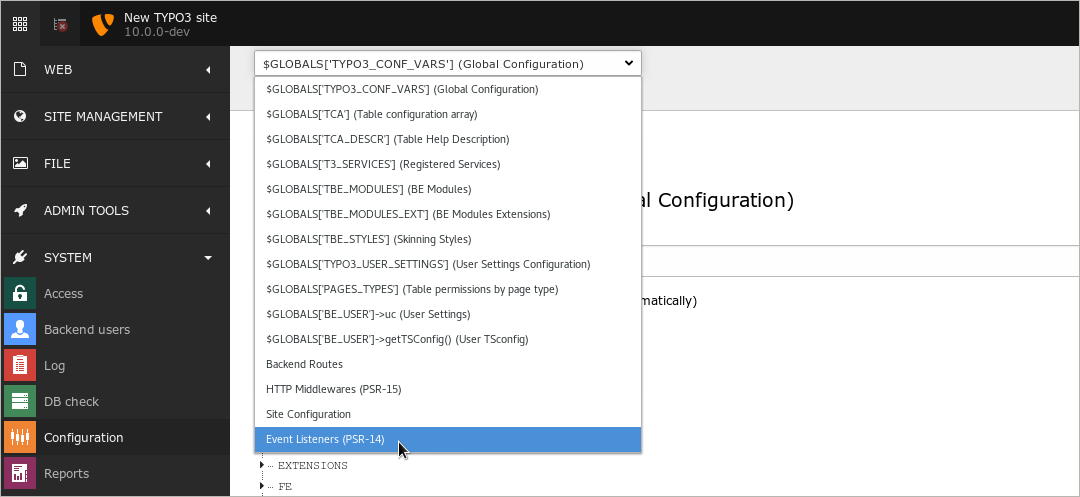
\includegraphics[width=0.70\linewidth]{ChangesForDevelopers/88770-PSR14-EventDispatcher.png}
	\end{figure}

\end{frame}


% ------------------------------------------------------------------------------
% Feature | 88769 | Introduce a generic EventDispatcher based on PSR-14
% Feature | 88770 | Add PSR-14 EventDispatcher logic based on DI

\begin{frame}[fragile]
	\frametitle{Changes for Developers}
	\framesubtitle{Event Dispatching (4)}

	% decrease font size for code listing
	\lstset{basicstyle=\tiny\ttfamily}

	\begin{itemize}
		\item Best practices:

			\begin{itemize}
				\item Add only one Listener per PHP class and use \texttt{\_\_invoke()} as the method name.
				\item Add "\texttt{Event}" suffix to the class name when creating a new Event PHP class.
				\item Move the Event PHP class file to an appropriate folder e.g. \texttt{Classes/Database/Event}.
				\item Use dependency injection in form of a constructor argument to receive the
					EventDispatcher object if possible.
			\end{itemize}

		\item Additional note:\newline
			\small
				Events provided by the TYPO3 core follow TYPO3's deprecation policy, except for its constructor
				arguments which may vary.
			\normalsize

	\end{itemize}

\end{frame}

% ------------------------------------------------------------------------------
% Feature | 88799 | Use PSR-3 interface for logging

\begin{frame}[fragile]
	\frametitle{Changes for Developers}
	\framesubtitle{PSR-3 Logging Interface}

	\begin{itemize}
		\item TYPO3's Logging Framework (in particular LogLevel and LogManager) now uses the
			\href{https://www.php-fig.org/psr/psr-3/}{PSR-3 Logger Interface}.

		\item PSR-3 is a standardized method that allows libraries to receive a
			\texttt{Psr\textbackslash
				Log\textbackslash
				LoggerInterface} object and to write logs to it in a simple and universal way.

			\item This lets developers use custom loggers and to interact with other
				logging systems.

	\end{itemize}

\end{frame}

% ------------------------------------------------------------------------------
% Breaking | 88182 | jsfunc.inline.js has been dropped
% Breaking | 88427 | jsfunc.evalfield.js has been removed
% Breaking | 88667 | Removed additionalJavaScriptSubmit from FormEngine
% Deprecation | 88433 | Deprecate top.openUrlInWindow

\begin{frame}[fragile]
	\frametitle{Changes for Developers}
	\framesubtitle{JavaScript Options and Functions (1)}

	\begin{itemize}
		\item The following JavaScript files have been removed:

			\begin{itemize}
				\item \texttt{jsfunc.inline.js}
				\item \texttt{jsfunc.evalfield.js}
			\end{itemize}

			\begin{itemize}\smaller
				\item[\ding{228}] Use \texttt{TYPO3/CMS/Backend/FormEngineValidation} instead.
			\end{itemize}\normalsize

		\item Additional submit handlers could previously be added by the option \texttt{additionalJavaScriptSubmit}.
			This option has been removed.

			\begin{itemize}\smaller
				\item[\ding{228}] Create and register an AMD module instead.
			\end{itemize}\normalsize

		\item The global JavaScript function \texttt{top.openUrlInWindow()} has been marked deprecated.

	\end{itemize}

\end{frame}

% ------------------------------------------------------------------------------
% Breaking | 88411 | TBE_EDITOR.typo3form removed
% Deprecation | 88432 | Replaced md5js with an AMD module
% Deprecation | 88428 | top.rawurlencode and top.str_replace
% Deprecation | 88651 | Replace TYPO3/CMS/Backend/SplitButtons with TYPO3/CMS/Backend/DocumentSaveActions

\begin{frame}[fragile]
	\frametitle{Changes for Developers}
	\framesubtitle{JavaScript Options and Functions (2)}

	\begin{itemize}

		\item The global object \texttt{TBE\_EDITOR.typo3form} and its backward layers \texttt{typo3FormFieldSet}
			and \texttt{typo3FormFieldGet} have been removed.

		\item File \texttt{md5.js} has been marked deprecated.

			\begin{itemize}\smaller
				\item[\ding{228}] Load the AMD module \texttt{TYPO3/CMS/Backend/Hashing/Md5} via RequireJS instead.
			\end{itemize}\normalsize

		\item The following global JavaScript functions have been marked deprecated:

		\begin{itemize}
			\item \texttt{top.rawurlencode()}
			\item \texttt{top.str\_replace()}
		\end{itemize}

		\item Module \texttt{TYPO3/CMS/Backend.SplitButtons} has been deprecated.

			\begin{itemize}\smaller
				\item[\ding{228}] Use \texttt{TYPO3/CMS/Backend/DocumentSaveActions} instead.
			\end{itemize}\normalsize

 	\end{itemize}

\end{frame}

% ------------------------------------------------------------------------------
% Important | 87894 | Removed PHP Dependency algo26-matthiasidna-convert

\begin{frame}[fragile]
	\frametitle{Changes for Developers}
	\framesubtitle{UTF-8-based Domains}

	\begin{itemize}
		\item PHP has native functions to convert domains from UTF-8 into IDNA ASCII form (“punicode”),
			for example \href{https://www.php.net/manual/en/function.idn-to-ascii.php}{idn\_to\_ascii()}.

		\item These can be used directly if the PHP extension
			"\href{https://www.php.net/manual/en/book.intl.php}{intl}" is installed.

		\item If the PHP extension is not installed, the package \texttt{symfony/polyfill-intl-idn}
			provides the functions now.

		\item Previously, the package \texttt{algo26-matthias/idna-convert} was used which has been removed now.

	\end{itemize}

\end{frame}

% ------------------------------------------------------------------------------
% Feature | 87665 | Introduce BitSet class

\begin{frame}[fragile]
	\frametitle{Changes for Developers}
	\framesubtitle{BitSet Class}

	% decrease font size for code listing
	\lstset{basicstyle=\tiny\ttfamily}

	\begin{itemize}
		\item New class has been introduced to efficiently handle boolean flags:\newline
			\texttt{TYPO3\textbackslash
				CMS\textbackslash
				Core\textbackslash
				Type\textbackslash
				BitSet}

		\item For example:

\begin{lstlisting}
define('PERMISSIONS_NONE', 0b0); // 0
define('PERMISSIONS_PAGE_SHOW', 0b1); // 1
define('PERMISSIONS_PAGE_EDIT', 0b10); // 2
define('PERMISSIONS_PAGE_DELETE', 0b100); // 4
define('PERMISSIONS_PAGE_NEW', 0b1000); // 8
define('PERMISSIONS_CONTENT_EDIT', 0b10000); // 16
define('PERMISSIONS_ALL', 0b11111); // 31

$bitSet = new \TYPO3\CMS\Core\Type\BitSet(PERMISSIONS_PAGE_SHOW | PERMISSIONS_PAGE_NEW);
$bitSet->get(PERMISSIONS_PAGE_SHOW); // true
$bitSet->get(PERMISSIONS_CONTENT_EDIT); // false
\end{lstlisting}

	\end{itemize}

\end{frame}

% ------------------------------------------------------------------------------
% Important | 87516 | Remove Core HTTP Request Handler Interface

\begin{frame}[fragile]
	\frametitle{Changes for Developers}
	\framesubtitle{Request Handler (1)}

	\begin{itemize}
		\item The following internal interface has been removed
			in favor of PSR-15 request handler and middleware interfaces:\newline
			\texttt{TYPO3\textbackslash
				CMS\textbackslash
				Core\textbackslash
				Http\textbackslash
				RequestHandlerInterface}

	\end{itemize}

\end{frame}

% ------------------------------------------------------------------------------
% Breaking | 88687 | Configure extbase request handlers via PHP

\begin{frame}[fragile]
	\frametitle{Changes for Developers}
	\framesubtitle{Request Handler (2)}

	% decrease font size for code listing
	\lstset{basicstyle=\tiny\ttfamily}

	\begin{itemize}
		\item The configuration of Extbase request handlers is no longer possible with TypoScript.

		\smaller\textbf{Old} method in TypoScript:\normalsize
\begin{lstlisting}
config.tx_extbase {
  mvc {
    requestHandlers {
      Vendor\Example\Mvc\Web\FrontendRequestHandler = Vendor\Example\Mvc\Web\FrontendRequestHandler
    }
  }
}
\end{lstlisting}

		\smaller\textbf{New} method in file \texttt{Configuration/Extbase/RequestHandlers.php}:\normalsize
\begin{lstlisting}
<?php
declare(strict_types = 1);

return [
  \Vendor\Example\Mvc\Web\FrontendRequestHandler::class,
];
\end{lstlisting}

	\end{itemize}

\end{frame}


% ------------------------------------------------------------------------------
% Deprecation | 88366 | Default caching framework cache names changed

\begin{frame}[fragile]
	\frametitle{Changes for Developers}
	\framesubtitle{Caching Framework}

	% decrease font size for code listing
	\lstset{basicstyle=\tiny\ttfamily}

	\begin{itemize}
		\item The following caches have been renamed:

			\begin{itemize}\smaller
				\item \texttt{cache\_core} \textrightarrow\hspace{0.1cm}\texttt{core}
				\item \texttt{cache\_hash} \textrightarrow\hspace{0.1cm}\texttt{hash}
				\item \texttt{cache\_pages} \textrightarrow\hspace{0.1cm}\texttt{pages}
				\item \texttt{cache\_pagesection} \textrightarrow\hspace{0.1cm}\texttt{pagesection}
				\item \texttt{cache\_runtime} \textrightarrow\hspace{0.1cm}\texttt{runtime}
				\item \texttt{cache\_rootline} \textrightarrow\hspace{0.1cm}\texttt{rootline}
				\item \texttt{cache\_imagesizes} \textrightarrow\hspace{0.1cm}\texttt{imagesizes}
			\end{itemize}\normalsize

		\item New method to access the caches:

\begin{lstlisting}
OLD:
$cacheManager->getCache('cache_core').

NEW:
$cacheManager->getCache('core')
\end{lstlisting}

		\item The prefix \texttt{cf\_} has been removed from the database tables.
	\end{itemize}

\end{frame}

% ------------------------------------------------------------------------------
% Deprecation | 87550 | Use controller classes when registering plugins/modules

\begin{frame}[fragile]
	\frametitle{Changes for Developers}
	\framesubtitle{Extbase and Fluid (1)}

	% decrease font size for code listing
	\lstset{basicstyle=\tiny\ttfamily}

	\begin{itemize}
		\item Registering plugins/modules require fully-qualified class names now

			\begin{itemize}\smaller
				\item \texttt{\textbackslash
					TYPO3\textbackslash
					CMS\textbackslash
					Extbase\textbackslash
					Utility\textbackslash
					ExtensionUtility::configurePlugin()}
				\item \texttt{\textbackslash
					TYPO3\textbackslash
					CMS\textbackslash
					Extbase\textbackslash
					Utility\textbackslash
					ExtensionUtility::registerModule()}
			\end{itemize}\normalsize

		\item Also omit vendor name in the extension name (first argument).

			\begin{itemize}\smaller
				\item[\ding{228}] Use "\texttt{ExampleBlog}" instead of "\texttt{Vendor.ExampleBlog}".
			\end{itemize}

		\item For example:

\begin{lstlisting}
\TYPO3\CMS\Extbase\Utility\ExtensionUtility::configurePlugin(
  'ExampleBlog', // previously: 'Vendor.ExampleBlog'
  'pi1',
  [
    \Vendor\Example\Controller\BlogController::class => 'list,update,delete'
  ],
  [
    \Vendor\Example\Controller\BlogController::class => 'list,update,delete'
  ]
);
\end{lstlisting}

	\end{itemize}

\end{frame}

% ------------------------------------------------------------------------------
% Breaking | 87627 | Remove Property extensionName of AbstractController

\begin{frame}[fragile]
	\frametitle{Changes for Developers}
	\framesubtitle{Extbase and Fluid (2)}

	\begin{itemize}
		\item Property \texttt{extensionName} of AbstractController has been removed.

			\begin{itemize}\smaller
				\item[\ding{228}] Use \texttt{\textbackslash
					TYPO3\textbackslash
					CMS\textbackslash
					Extbase\textbackslash
					Mvc\textbackslash
					Request::getControllerExtensionName()} instead.
			\end{itemize}\normalsize

	\end{itemize}

\end{frame}

% ------------------------------------------------------------------------------
% Feature | 87457 | Use symfony/propertyinfo to gather doc block information

\begin{frame}[fragile]
	\frametitle{Changes for Developers}
	\framesubtitle{Extbase and Fluid (3)}

	% decrease font size for code listing
	\lstset{basicstyle=\tiny\ttfamily}

	\begin{itemize}
		\item Extbase models now support non fully-qualified class names in DocBlocks.

\begin{lstlisting}
use TYPO3\CMS\Extbase\Persistence\ObjectStorage;
use ExtbaseTeam\BlogExample\Domain\Model\Comment;

class Post
{
  /**
   * @var ObjectStorage<Comment>
   */
  public $comments;
}
\end{lstlisting}

	\end{itemize}

\end{frame}

% ------------------------------------------------------------------------------
% Breaking | 87957 | Validators are not registered automatically in Extbase anymore

\begin{frame}[fragile]
	\frametitle{Changes for Developers}
	\framesubtitle{Extbase and Fluid (4)}

	% decrease font size for code listing
	\lstset{basicstyle=\tiny\ttfamily}

	\begin{itemize}
		\item Validators are not registered automatically in Extbase anymore.
		\item For a model named
			\small\texttt{Vendor\textbackslash
				Example\textbackslash
				Domain\textbackslash
				Model\textbackslash
				Blog}\normalsize,\newline
			Extbase automatically used the validator
			\small\texttt{Vendor\textbackslash
				Example\textbackslash
				Domain\textbackslash
				Validator\textbackslash
				BlogValidator}\normalsize

		\item Validators need to be registered manually now:

\begin{lstlisting}
use Vendor\Example\Domain\Model\Blog;
use TYPO3\CMS\Extbase\Annotation as Extbase;
use TYPO3\CMS\Extbase\Mvc\Controller\ActionController;

class BlogController extends ActionController
{
  /**
   * @Extbase\Validate(param="blog", validator="Vendor\Example\Domain\Validator\BlogValidator")
   */
  public function showAction(Blog $blog)
  {
    // ...
  }
}
\end{lstlisting}

	\end{itemize}

\end{frame}

% ------------------------------------------------------------------------------
% Breaking | 87623 | Replace config.persistence.classes typoscript configuration (1)

\begin{frame}[fragile]
	\frametitle{Changes for Developers}
	\framesubtitle{Extbase and Fluid (5) - Class Mapping}

	% decrease font size for code listing
	\lstset{basicstyle=\tiny\ttfamily}

	\begin{itemize}
		\item Persistence related class mapping using TypoScript is no longer supported:

\begin{lstlisting}
config.tx_example_blog {
  persistence {
    classes {
      Vendor\Example\Domain\Model\Author {
        mapping {
          tableName = fe_users
          columns.name.mapOnProperty = fullname
        }
      }
    }
  }
}
\end{lstlisting}

	\end{itemize}

\end{frame}

% ------------------------------------------------------------------------------
% Breaking | 87623 | Replace config.persistence.classes typoscript configuration (2)

\begin{frame}[fragile]
	\frametitle{Changes for Developers}
	\framesubtitle{Extbase and Fluid (6) - Class Mapping}

	% decrease font size for code listing
	\lstset{basicstyle=\tiny\ttfamily}

	\begin{itemize}
		\item The mapping needs to be implemented in a PHP file \texttt{Configuration/Extbase/Persistence/Classes.php}:

\begin{lstlisting}
<?php
declare(strict_types = 1);

return [
  \Vendor\Example\Domain\Model\Author::class => [
    'tableName' => 'fe_users',
    'properties' => [
      'fullname' => [
        'fieldName' => 'name'
      ]
    ]
  ]
];
\end{lstlisting}

		\begin{itemize}\smaller
			\item[\ding{228}] Note that property name and DB field have swapped!\newline
				Previously:\tabto{1.6cm}\texttt{<db-field>.mapOnProperty = <property>}\newline
				New:\tabto{1.6cm}\texttt{properties.<property>.fieldname = <db-field>}
		\end{itemize}\normalsize

	\end{itemize}

\end{frame}

% ------------------------------------------------------------------------------
% Breaking | 87594 | Harden Extbase

\begin{frame}[fragile]
	\frametitle{Changes for Developers}
	\framesubtitle{Extbase and Fluid (7)}

	% decrease font size for code listing
	\lstset{basicstyle=\smaller\ttfamily}

	\begin{itemize}
		\item Class files now feature the "strict types" mode and type hints for scalars

\begin{lstlisting}
<?php
declare(strict_types=1);
\end{lstlisting}

		% Method signatures in Extbase classes have been updated.
		\item This results in fatal PHP errors if the method signatures in custom
			extensions are not compatible with the interfaces and/or parent classes.

		\item See \href{https://forge.typo3.org/issues/87594}{forge \#87594}
			for a complete list of files and their changes.

		\item This task is still work in progress and further changes will be made.

	\end{itemize}

\end{frame}

% ------------------------------------------------------------------------------
% Breaking | 87937 | TCA option selicon_field_path removed
% Breaking | 87989 | TCA option setToDefaultOnCopy removed
% Breaking | 87936 | TCA for sys_history removed

\begin{frame}[fragile]
	\frametitle{Changes for Developers}
	\framesubtitle{TCA Changes}

	\begin{itemize}
		\item The following TCA options have been removed:

			\begin{itemize}
				\item \texttt{\$TCA[\$tableName]['ctrl']['selicon\_field\_path']}
				\item \texttt{\$TCA[\$tableName]['ctrl']['setToDefaultOnCopy']}
			\end{itemize}

			\begin{itemize}\smaller
				\item[\ding{228}] When copying records, a DataHandler should be used to reset fields.
			\end{itemize}\normalsize

		\item The entire TCA of \texttt{sys\_history} has been removed and the database field \texttt{pid} dropped.
			Accessing \texttt{\$GLOBALS['TCA']['sys\_history']} now triggers a PHP warning.

	\end{itemize}

\end{frame}

% ------------------------------------------------------------------------------
% Breaking | 88527 | Overriding custom values in User Authentication derivatives

\begin{frame}[fragile]
	\frametitle{Changes for Developers}
	\framesubtitle{User Authentication Classes/Services (1)}

	\begin{itemize}
		\item The following abstract class has been restructured:\newline
			\small\texttt{TYPO3\textbackslash
				CMS\textbackslash
				Core\textbackslash
				Authentication\textbackslash
				AbstractUserAuthentication}\normalsize
		\item This also includes the following two direct sub-classes:

			\begin{itemize}
				\item \texttt{BackendUserAuthentication}
				\item \texttt{FrontendUserAuthentication}
			\end{itemize}

		\item This change affects the properties:

			\begin{itemize}
				\item \texttt{sessionTimeout}
				\item \texttt{gc\_time}
				\item \texttt{sessionDataLifetime}
				\item \texttt{loginType}
			\end{itemize}

	\end{itemize}

\end{frame}

% ------------------------------------------------------------------------------
% Breaking | 88646 | Removed inheritance of AbstractService from AbstractAuthenticationService

\begin{frame}[fragile]
	\frametitle{Changes for Developers}
	\framesubtitle{User Authentication Classes/Services (2)}

	\begin{itemize}

		\item The following class does not inherit from
			\smaller\texttt{AbstractService}\normalsize\hspace{0.1cm}
			anymore:
			\smaller\texttt{\textbackslash
				TYPO3\textbackslash
				CMS\textbackslash
				Core\textbackslash
				Authentication\textbackslash
				AbstractAuthenticationService}\normalsize

		\item This possibly affects some of the hooks and custom authentication providers available.

		\item Developers are advised to review their custom authentication services and update
			their code if required.

	\end{itemize}

\end{frame}

% ------------------------------------------------------------------------------
% Deprecation | 87882 | File related controllers moved to EXT:filelist

\begin{frame}[fragile]
	\frametitle{Changes for Developers}
	\framesubtitle{Filelist Controllers}

	\begin{itemize}
		\item The following controllers have been moved to \texttt{EXT:filelist}:

			\begin{itemize}\small
				\item \texttt{CreateFolderController}
				\item \texttt{EditFileController}
				\item \texttt{FileUploadController}
				\item \texttt{RenameFileController}
				\item \texttt{ReplaceFileController}
			\end{itemize}\normalsize

		\item As a result, their namespace changed to\newline
			\texttt{\textbackslash
				TYPO3\textbackslash
				CMS\textbackslash
				Filelist\textbackslash
				Controller\textbackslash
				File}

		\vspace{0.2cm}

		\small
			Note: Use the TYPO3 FAL as API and add your own functionality
			with your own controller instead of reusing the \textbf{internal}
			controllers listed above.
		\normalsize

	\end{itemize}

\end{frame}

% ------------------------------------------------------------------------------
% Deprecation | 88499 | BackendUtility::getViewDomain()

\begin{frame}[fragile]
	\frametitle{Changes for Developers}
	\framesubtitle{Frontend Preview URL}

	% decrease font size for code listing
	\lstset{basicstyle=\tiny\ttfamily}

	\begin{itemize}
		\item The following static method has been marked deprecated:\newline
			\smaller\texttt{\textbackslash
				TYPO3\textbackslash
				CMS\textbackslash
				Backend\textbackslash
				Utility\textbackslash
				BackendUtility::getViewDomain()}\normalsize

		\item Substitute the method by directly detecting a site based on a given page ID in the TYPO3 backend.
		\item For example:

\begin{lstlisting}
$pageId = 123;
$site = GeneralUtility::makeInstance(SiteFinder::class)->getSiteByPageId($pageId);
$url = $site->getRouter()->generateUri($pageId, ['type' => 13]);
\end{lstlisting}

	\end{itemize}

\end{frame}

% ------------------------------------------------------------------------------
% Deprecation | 88406 | setCacheHash/noCacheHash options in ViewHelpers and UriBuilder

\begin{frame}[fragile]
	\frametitle{Changes for Developers}
	\framesubtitle{cHash in UriBuilder and ViewHelpers}

	% decrease font size for code listing
	\lstset{basicstyle=\smaller\ttfamily}

	\begin{itemize}
		\item The following two Extbase UriBuilder methods have been deprecated:

			\begin{itemize}
				\item \texttt{UriBuilder->setUseCacheHash()}
				\item \texttt{UriBuilder->getUseCacheHash()}
			\end{itemize}

		\item This also impacts a number of Fluid ViewHelpers:
	\end{itemize}
	\vspace{-0.4cm}
	\begin{columns}[T]
		\begin{column}{.05\textwidth}
		\end{column}
		\begin{column}{.45\textwidth}
			\begin{itemize}\smaller
				\item \texttt{f:form}
				\item \texttt{f:link.action}
				\item \texttt{f:link.page}
				\item \texttt{f:link.typolink}
				\item \texttt{f:uri.action}
			\end{itemize}\normalsize
		\end{column}
		\begin{column}{.45\textwidth}
			\begin{itemize}\smaller
				\item \texttt{f:uri.page}
				\item \texttt{f:uri.typolink}
				\item \texttt{f:widget.link}
				\item \texttt{f:widget.uri}
			\end{itemize}\normalsize
		\end{column}
	\end{columns}
	\vspace{0.2cm}
	\begin{itemize}
		\item ...as well as the TypoLink option "\texttt{useCacheHash}".
	\end{itemize}

\end{frame}

% ------------------------------------------------------------------------------
% Breaking | 88540 | Changed Request Workflow for Frontend Requests

\begin{frame}[fragile]
	\frametitle{Changes for Developers}
	\framesubtitle{Frontend Request Workflow (1)}

	% decrease font size for code listing
	\lstset{basicstyle=\smaller\ttfamily}

	\begin{itemize}
		\item The Frontend Request Workflow has been reworked significantly.

		\item Components involved are all built using PSR-15 middlewares, the PSR-15 Request Handler,
			and the global TypoScriptFrontendController (TSFE) since TYPO3 v9.

		\item This impacts custom code, if the following hook and a frontend session is used:\newline
			{\fontsize{7}{8}\selectfont\texttt{\$GLOBALS['TYPO3\_CONF\_VARS']['SC\_OPTIONS']['tslib/class.tslib\_fe.php']['hook\_eofe']}}

			\begin{itemize}\smaller
				\item[\ding{228}] Use a PSR-15 middleware instead of a hook, or explicitly call \texttt{storeSessionData}
				within the hook in PHP.
			\end{itemize}\normalsize

	\end{itemize}

\end{frame}

% ------------------------------------------------------------------------------
% Breaking | 88498 | Global data for TimeTracker statistics removed

\begin{frame}[fragile]
	\frametitle{Changes for Developers}
	\framesubtitle{Frontend Request Workflow (2)}

	% decrease font size for code listing
	\lstset{basicstyle=\smaller\ttfamily}

	\begin{itemize}
		\item The following global variables have been removed:

			\begin{itemize}
				\item \texttt{\$GLOBALS['TYPO3\_MISC']['microtime\_start']}
				\item \texttt{\$GLOBALS['TYPO3\_MISC']['microtime\_end']}
				\item \texttt{\$GLOBALS['TYPO3\_MISC']['microtime\_BE\_USER\_start']}
				\item \texttt{\$GLOBALS['TYPO3\_MISC']['microtime\_BE\_USER\_end']}
			\end{itemize}

		\item The TYPO3 core used them in the Admin Panel and HTTP header for example.

			\begin{itemize}\smaller
				\item[\ding{228}] Use \texttt{TimeTracker->finish()} instead.
			\end{itemize}\normalsize

	\end{itemize}

\end{frame}


% ------------------------------------------------------------------------------
% Deprecation | 88569 | Locales::initialize() in favor of regular singleton instance
% Deprecation | 88473 | TypoScriptFrontendController->settingLocale

\begin{frame}[fragile]
	\frametitle{Changes for Developers}
	\framesubtitle{Locales (1)}

	\begin{itemize}
		\item Method \texttt{Locales::initialize()} has been marked deprecated.

			\begin{itemize}\smaller
				\item[\ding{228}] Use \texttt{GeneralUtility::makeInstance(Locales::class)} or
				dependency injection to fetch an instance of the class \texttt{Locales} instead.
			\end{itemize}\normalsize

		\item Functionality of the following method has been marked deprecated:\newline
			\texttt{TypoScriptFrontendController->settingLocale()}.

			\begin{itemize}\smaller
				\item[\ding{228}] Function is now available as
				{\fontsize{8}{8} \selectfont \texttt{Locales::setSystemLocaleFromSiteLanguage()}.}
			\end{itemize}\normalsize

	\end{itemize}

\end{frame}

% ------------------------------------------------------------------------------
% Deprecation | 88559 | TSFE->sys_language_isocode

\begin{frame}[fragile]
	\frametitle{Changes for Developers}
	\framesubtitle{Locales (2)}

	\begin{itemize}
		\item Public property \texttt{TypoScriptFrontendController->sys\_language\_isocode}
			has been marked deprecated.

			\begin{itemize}\smaller
				\item[\ding{228}] Access the property via \texttt{SiteLanguage->getTwoLetterIsoCode()}
				and \texttt{sitelanguage:twoLetterIsoCode} instead.
			\end{itemize}\normalsize

	\end{itemize}

\end{frame}

% ------------------------------------------------------------------------------
% Breaking | 88458 | Removed Frontend Track User ftu functionality

\begin{frame}[fragile]
	\frametitle{Changes for Developers}
	\framesubtitle{Frontend Track User}

	\begin{itemize}

		\item This following public properties of class\newline
			\smaller\texttt{\textbackslash
				TYPO3\textbackslash
				CMS\textbackslash
				Core\textbackslash
				Authentication\textbackslash
				AbstractUserAuthentication}
			\normalsize\newline
			have been removed:

			\begin{itemize}\smaller
				\item \texttt{AbstractUserAuthentication->get\_name}
				\item \texttt{AbstractUserAuthentication->getFallBack}
				\item \texttt{AbstractUserAuthentication->getMethodEnabled}
				\item \texttt{AbstractUserAuthentication->get\_URL\_ID}
			\end{itemize}\normalsize

		\item Also the property \texttt{getMethodUrlIdToken} of class\newline
			\smaller\texttt{\textbackslash
				TYPO3\textbackslash
				CMS\textbackslash
				Frontend\textbackslash
				Controller\textbackslash
				TypoScriptFrontendController}.
			\normalsize

		\item And the TypoScript setting \texttt{config.ftu},
			as well as the global configuration
			{\fontsize{8}{8} \selectfont \texttt{\$GLOBALS['TYPO3\_CONF\_VARS']['FE']['get\_url\_id\_token']}.}

	\end{itemize}

\end{frame}

% ------------------------------------------------------------------------------
% Breaking | 87305 | Use constructor injection in DataMapper

\begin{frame}[fragile]
	\frametitle{Changes for Developers}
	\framesubtitle{Constructor Injection in DataMapper}

	\begin{itemize}

		\item The following class now uses constructor injection rather than setter injection:
			\smaller
				\texttt{\textbackslash
					TYPO3\textbackslash
					CMS\textbackslash
					Extbase\textbackslash
					Persistence\textbackslash
					Generic\textbackslash
					Mapper\textbackslash
					DataMapper}
			\normalsize

			\begin{itemize}\smaller
				\item[\ding{228}] Avoid \texttt{GeneralUtility::makeInstance()} and \texttt{ObjectManager->get()}.
				\item[\ding{228}] Use dependency injection instead (preferably constructor injection).
			\end{itemize}\normalsize

	\end{itemize}

\end{frame}

% ------------------------------------------------------------------------------
% Feature | 88791 | Introduce PreviewAspect in Context

\begin{frame}[fragile]
	\frametitle{Changes for Developers}
	\framesubtitle{Context API (1)}

	% decrease font size for code listing
	\lstset{basicstyle=\tiny\ttfamily}

	\begin{itemize}

		\item The Context API features a new aspect "\texttt{frontend.preview}"
			that can be used to determine if the frontend is in preview mode:

\begin{lstlisting}
GeneralUtility::makeInstance(Context::class)
  ->getPropertyFromAspect('frontend.preview', 'isPreview');
\end{lstlisting}

		\item This aspect replaces the following property which is marked deprecated now:
			\small\texttt{TypoScriptFrontendController->fePreview}\normalsize

	\end{itemize}

\end{frame}

% ------------------------------------------------------------------------------
% Feature | 88792 | Add TypoScriptAspect to handle TypoScript Rendering Context settings
% Deprecation | 88792 | forceTemplateParsing in TSFE and TemplateService has been deprecated

\begin{frame}[fragile]
	\frametitle{Changes for Developers}
	\framesubtitle{Context API (2)}

	% decrease font size for code listing
	\lstset{basicstyle=\tiny\ttfamily}

	\begin{itemize}

		\item Another new aspect \texttt{TypoScriptAspect} can be used to manipulate/check if
			TemplateRendering is forced.

		\item The setting \texttt{forceTemplateParsing} (TSFE and TemplateService) has been deprecated.
			The Context API should be used instead:

\begin{lstlisting}
GeneralUtility::makeInstance(Context::class)
  ->getPropertyFromAspect('typoscript', 'forcedTemplateParsing');

$context->setAspect(
  'typoscript',
  GeneralUtility::makeInstance(TypoScriptAspect::class, true)
);
\end{lstlisting}

	\end{itemize}

\end{frame}

% ------------------------------------------------------------------------------
% Breaking | 88525 | Remove “createDirs” directive of extension installation / ext_emconf.php
% Breaking | 87511 | Remove $viewFormatToObjectNameMap property
% Breaking | 87511 | Remove $namespacesViewObjectNamePattern property
% Feature | 87726 | Extend Frontend Login Controller Hook To Validate Password

\begin{frame}[fragile]
	\frametitle{Changes for Developers}
	\framesubtitle{Miscellaneous (1)}

	\begin{itemize}
		\item Directive \texttt{createDirs} in file \texttt{ext\_emconf.php} not supported anymore.

			\begin{itemize}\smaller
				\item[\ding{228}] Folders will not be created automatically during extension installation.
			\end{itemize}\normalsize

		\item The following two properties in class
			\texttt{TYPO3\textbackslash
				CMS\textbackslash
				Extbase\textbackslash
				Mvc\textbackslash
				Controller\textbackslash
				ActionController}\newline
			have been removed:

			\begin{itemize}
				\item \texttt{\$namespacesViewObjectNamePattern}
				\item \texttt{\$viewFormatToObjectNameMap}
			\end{itemize}

		\item The following existing hook has been extended and can now
			also be used to validate passwords:\newline
			{\fontsize{8}{10} \selectfont \texttt{\$GLOBALS['TYPO3\_CONF\_VARS']['EXTCONF']['felogin']['password\_changed']}}

	\end{itemize}

\end{frame}

% ------------------------------------------------------------------------------
% Deprecation | 87613 | Deprecate /TYPO3/CMS/Extbase/Utility/TypeHandlingUtility::hex2bin
% Deprecation | 88554 | Deprecated methods in VersionNumberUtility

\begin{frame}[fragile]
	\frametitle{Changes for Developers}
	\framesubtitle{Miscellaneous (2)}

	\begin{itemize}

		\item The following method has been marked deprecated:\newline
			\smaller\texttt{\textbackslash
				TYPO3\textbackslash
				CMS\textbackslash
				Extbase\textbackslash
				Utility\textbackslash
				TypeHandlingUtility::hex2bin()}\normalsize

			\begin{itemize}\smaller
				\item[\ding{228}] Use the native PHP function \href{https://www.php.net/manual/en/function.hex2bin.php}{hex2bin()} instead.
			\end{itemize}\normalsize

		\item The following methods of class
			\smaller\texttt{\textbackslash
				TYPO3\textbackslash
				CMS\textbackslash
				Core\textbackslash
				Utility\textbackslash
				VersionNumberUtility}\normalsize\newline
			have been marked deprecated:

			\begin{itemize}
				\item \texttt{convertIntegerToVersionNumber()}
				\item \texttt{splitVersionRange()}
				\item \texttt{raiseVersionNumber()}
			\end{itemize}

			\begin{itemize}\smaller
				\item[\ding{228}] Implement the methods as custom code.
			\end{itemize}\normalsize

	\end{itemize}

\end{frame}

% ------------------------------------------------------------------------------
% Feature | 86964 | Allow getting class property default value
% Deprecation | 82669 | Streamline Backend route path inconsistencies

\begin{frame}[fragile]
	\frametitle{Changes for Developers}
	\framesubtitle{Miscellaneous (3)}

	% decrease font size for code listing
	\lstset{basicstyle=\tiny\ttfamily}

	\begin{itemize}
		\item It is now possible to get the default value of a class property
			when using the ReflectionService.

\begin{lstlisting}
$property = GeneralUtility::makeInstance(ReflectionService::class)
  ->getClassSchema(MyClass::class)
  ->getProperty('myProperty');
\end{lstlisting}

		\item Backend routes to modules without path configurations are now named\newline
			"\texttt{/module/<main-module>/<sub-module>}" by default\newline
			\small
				(for example: "\texttt{/module/web/ts}".)
			\normalsize

		\item Old routes still work (e.g. "\texttt{/web/ts/}") but this syntax will be removed in TYPO3 v11.

	\end{itemize}

\end{frame}

% ------------------------------------------------------------------------------
% Breaking | 88669 | FormEngine FormDataProvider parentPageTca removed
% Breaking | 88744 | Database fields related to CSS Styled Content removed
% Breaking | 88143 | Version-related database field “t3ver_id” removed
% Deprecation | 88746 | PageRepository PHP class moved from Frontend to Core Extension

\begin{frame}[fragile]
	\frametitle{Changes for Developers}
	\framesubtitle{Miscellaneous (4)}

	\begin{itemize}
		\item The FormEngine DataProvider \texttt{parentPageTca} has been removed.

			\begin{itemize}\smaller
				\item[\ding{228}] Developers can access \texttt{\$GLOBALS['TCA']['pages']} directly, instead of \texttt{\$result['parentPageTca']}.
			\end{itemize}\normalsize

		\item The following database fields have been removed:

			\begin{itemize}\smaller
				\item \texttt{tt\_content.spaceBefore} (replaced by field \texttt{space\_before\_class})
				\item \texttt{tt\_content.spaceAfter} (replaced by field \texttt{space\_after\_class})
				\item \texttt{pages.t3ver\_id} (unused since TYPO3 v9)
			\end{itemize}\normalsize

		\item The PHP class
			\texttt{\textbackslash
				TYPO3\textbackslash
				CMS\textbackslash
				Frontend\textbackslash
				Page\textbackslash
				PageRepository} has been moved from the "frontend" system extension into the core.

			\begin{itemize}\smaller
				\item Replace with class:
					\texttt{\textbackslash
						TYPO3\textbackslash
						CMS\textbackslash
						Core\textbackslash
						Domain\textbackslash
						Repository\textbackslash
						PageRepository}
			\end{itemize}\normalsize

	\end{itemize}

\end{frame}

% ------------------------------------------------------------------------------
% Breaking | 88574 | 4th parameter of PageRepository>enableFields removed
% Deprecation | 85895 | Deprecate File::_getMetaData()
% Deprecation | 88662 | Deprecated backend route xMOD_tximpexp

\begin{frame}[fragile]
	\frametitle{Changes for Developers}
	\framesubtitle{Miscellaneous (5)}

	\begin{itemize}

		\item 4th parameter of method \texttt{PageRepository->enableFields()} has been removed.

		\begin{itemize}\smaller
			\item[\ding{228}] If developers use a 4th parameter in this method call, which is set to "\textbf{false}", this can be removed safely.
			\item[\ding{228}] If it is set to "\textbf{true}", the code needs to be replaced with a separate instance of \texttt{PageRepository} with a custom \texttt{Context}.
		\end{itemize}\normalsize

		\item The internal method \texttt{File::\_getMetaData()}, which is used to fetch meta data of a file,
			has been marked deprecated.

			\begin{itemize}\smaller
				\item[\ding{228}] Use \texttt{\$fileObject->getMetaData()->get()} to fetch the meta data instead.
			\end{itemize}\normalsize

		\item The route identifier "\texttt{xMOD\_tximpexp}" has been marked deprecated.

			\begin{itemize}\smaller
				\item[\ding{228}] Use \texttt{tx\_impexp\_export} or \texttt{tx\_impexp\_import} depending on the use case.
			\end{itemize}\normalsize

	\end{itemize}

\end{frame}

% ------------------------------------------------------------------------------
% Breaking | 88496 | Method getSwitchableControllerActions has been removed
% Breaking | 87567 | Global variable $TBE_TEMPLATE removed
% Breaking | 88660 | $GLOBALS[T3_VAR] removed

\begin{frame}[fragile]
	\frametitle{Changes for Developers}
	\framesubtitle{Miscellaneous (6)}

	\begin{itemize}

		\item The following abstract method has been removed:\newline
			\smaller
				\texttt{\textbackslash
					TYPO3\textbackslash
					CMS\textbackslash
					Extbase\textbackslash
					Configuration\textbackslash
					AbstractConfigurationManager::}\newline
					\texttt{getSwitchableControllerActions()}
			\normalsize

			\begin{itemize}\smaller
				\item[\ding{228}] Use the new method name \texttt{getControllerConfiguration()} instead (same PHP class).
			\end{itemize}\normalsize

		\item The global variable \texttt{\$TBE\_TEMPLATE} has been removed, including
			the related PSR-15 middleware (which was marked as internal).

			\begin{itemize}\smaller
				\item[\ding{228}] Instantiate the DocumentTemplate class directly in the controller of the module.
				\item[\ding{228}] Migrate to ModuleTemplate which is available since TYPO3 v7.
			\end{itemize}\normalsize

		\item The global variable \texttt{\$GLOBALS['T3\_VAR']} has been removed.\newline

	\end{itemize}

\end{frame}

% ------------------------------------------------------------------------------
